\documentclass[hidelinks,a4paper,12pt]{article}
\usepackage[english]{babel}
\usepackage[utf8]{inputenc}
\usepackage{csquotes}
\usepackage{graphicx}
\usepackage{makecell}
\usepackage[margin=0.7in]{geometry}
\usepackage[T1]{fontenc}
\usepackage{mathptmx}
\usepackage{hyperref}
\hypersetup{
    colorlinks=false,
    linkcolor=blue,
    filecolor=magenta,      
    urlcolor=cyan,
}
\usepackage[normalem]{ulem}
\usepackage{xcolor}

\renewcommand\theadalign{bc}
\renewcommand\theadfont{\bfseries}
\renewcommand\theadgape{\Gape[4pt]}
\renewcommand\cellgape{\Gape[4pt]}
\graphicspath{ {./images/} }

\usepackage{comment}
  
\usepackage[backend=biber,style=numeric-comp,sorting=none,]{biblatex}
\addbibresource{references.bib} %Imports bibliography file

%opening
\title{Software Proposal Document for ....}
\author{Team Leader name, Second Name, Third Name, Fourth Name, Fifth Name \\
Supervised by: Dr. Essam Eliwa, Eng. Omar Magdy}


\begin{document}
\maketitle
\begin{table}[ht]

\caption{Document version history}
\begin{tabular}{|l|l|l|}
\hline
\thead{Proposal Version}    & \thead{Date} & \thead{Reason for Change}  \\ \hline
1.0 & 25-Feb-2023   & \makecell{Proposal First version’s specifications are defined}   \\ \hline
1.1 & 28-Feb-2023   & \makecell{System description updated} \\ \hline
\end{tabular}

\end{table}

\begin{table}[ht]
\begin{tabular}{cc}
\thead{GitHub:}    & {........................................................}   
\end{tabular}
\end{table}

\medskip

\begin{abstract}
The abstract should be concise and compelling, providing a compelling summary that encourages the reader to continue reading the full proposal document. It should briefly overview the proposed software project, including its purpose, scope, and critical features. It should give the reader a clear understanding of the project's objectives and benefits and any unique aspects that set it apart from similar software solutions.
The abstract should also include information about the software's target audience or user group and any relevant market or industry trends that make the project particularly timely.
In addition, the abstract may summarize key technical details such as the software's architecture, programming language, development methodology, and testing procedures. It may also mention any significant risks or challenges associated with the project and the strategies proposed to mitigate them.

To write a good abstract you can follow this guideline:

\begin{itemize}
    \item Introduction. In one sentence, what’s the topic? Phrase it in a way that your reader will understand the context.
    \item In one sentence, State the problem you tackle. What’s the key project challenge?
    \item Explain, in one or two sentences, how you plan to solve this problem.
    \item In one sentence, State the development process you intend to apply.
    \item In one sentence, what’s the key expected outcome of your project? (The proposed solution is a web application that will ........ )
\end{itemize}
(Word Limit 200).
PS. the abstract is the last thing you write in the document. 
\newpage
\end{abstract}
\medskip
\section{Introduction}
(The following is a sample guideline for MIU SE305 and CSC341 project proposal.)
\subsection{Background}
Please describe the big domain (context) for your problem then focus on some area inside this domain that match your interest. Use references to show your understanding of the topic and to give supporting evidence for your ideas.  For example for work related to Interior Design Management software you may reference \cite{shu2021application}. (Word Limit 200)

\subsection{Problem Statement}
Problem statements lead the reader from a shared context to the perception of a problem, and on to a proposed solution.
Three key points to get from this section are:\\
\begin{itemize}
    \item Context — Establish a context for your audience
    \item Problem — Define the problem within this context
    \item Solution — Propose a solution to this problem
\end{itemize}
\textbf{Example:}\\
(problem and its context)\\
A recent trend in the design of new aircraft is the addition of winglets, which are small fins attached to the ends of the main wing. After an aircraft has taken off and is cruising, winglets improve its performance by reducing the drag caused by the main wing. However, during the critical stages of aircraft takeoff and landing, the winglets cause two problems. First, they cause vibrations in the main wing, commonly called buffeting. Second, they cause the aircraft to lose some control of yaw, the motion of the nose right and left. In a study funded by NASA, the main wing of a DC-10 transport aircraft was outfitted with winglets, and it experienced significant buffeting during takeoff and landing.\\
(approach of the current research)\\ In our current project, we examine winglet-induced buffeting in three wing designs. We record buffeting and yaw under experimental wind-tunnel takeoff and landing conditions for (1) a wing without winglets, (2) another wing with conventional winglets, and (3) a wing with spheroid winglets. Our objective is to determine the degree to which differences between load lifts on the wings and their winglets during takeoff and landing are causing the performance problems we have described.

(scope of the proposed solution) In this study, we develop theoretical models of winglet load lifts and compare these to the lifts of wings and winglets actually recorded during testing conditions.
\subsection{Motivation}

Discuss the business needs for your project. \\
For this section consider answering the following questions:
\begin{enumerate}
\item Why is this problem interesting?
\item When and why does the problem occur?
\item What is the most current/successful solutions available now?
\item What are the possible improvements to current solutions?
\end{enumerate}

\section{Project Description}
Give a brief overview of your proposed project then list the initial requirements. A good requirement states something that is \textbf{necessary}, \textbf{verifiable}, and \textbf{attainable}. Even if it is verifiable and attainable if it is not necessary, it is not a good requirement \cite{hooks1994writing,ieee1998ieee,knauss2008}.
\\Use a figure such as in figure \ref{fig:overview} to show the proposed system.

\begin{figure}[h]
\centering
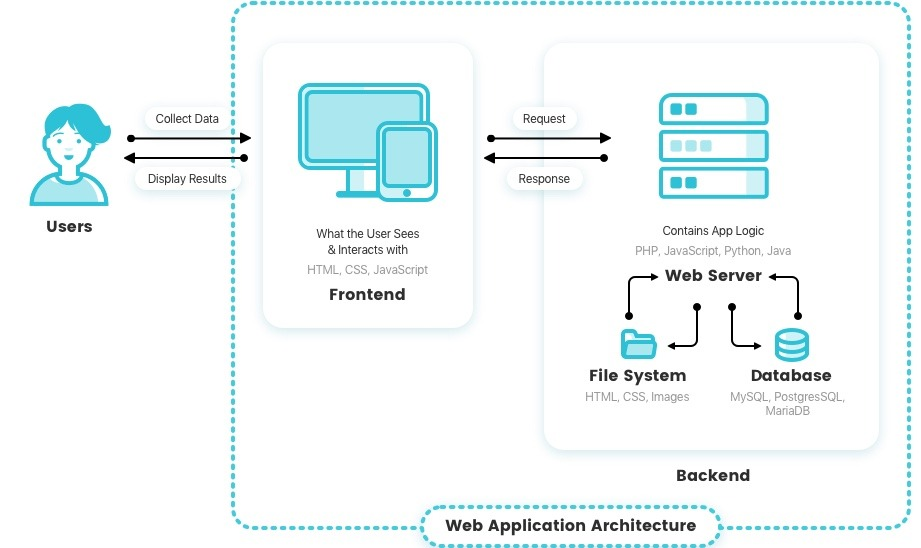
\includegraphics[width=0.8\linewidth]{images/web_app_Arch.jpeg}
\caption{web application architecture}
\label{fig:overview}
\end{figure}
\newpage

\subsection{Objectives}
Write as a minimum three statements that describe the “what” of your project. \\The concrete and measurable “what”. 
\\Aim to use the specific, measurable, assignable, realistic, and time-related (SMART) method for writing effective Objectives.
Examples of good Objectives:
\begin{itemize}
\item To reduce the number of clicks it takes for a user to reach the highest traffic page that the majority of our website users regularly visit (the member directory) from any point on the site to 2 clicks or less by the end of our design phase on June 1st.
\item To write the SRS document to meet with IEEE 830-1998 standard. SRS document will be delivered by April 2021.
\end{itemize}

\subsection{Stakeholder}
\subsubsection{Internal}
State who is the team leader. list all team members with their responsibilities
\subsubsection{External}
State who are the End Users and clients

\section{Similar System}
\subsection{Academic}

List down at least 1 paper from ACM or IEEE for similar work experience in the domain of your problem. Be sure that each paper you list include the following points

\begin{enumerate}
\item The main problem statement of the work.
\item How the researchers contributed to solve the problem
\item The dataset used by the researchers
\item What main results the researchers reach.
\item Criticize the paper
\item Figure/s of the work (if available)
\end{enumerate}

\subsection{Business Applications}
Describe available business applications in the market with figures.





\section{Project Management and Deliverables}
\subsection{Deliverables}
\begin{itemize}
\item What will the project produce? (program, reports, etc.)
\item Describe in brief detail the features of each deliverable.
\end{itemize}
\subsection{Tasks and Time Plan}
Use \textcolor{blue}{\href{https://trello.com/power-ups/58bd1f9aca72f48c8900574f}{Trello}} to create a time plan showing tasks and which team member is assigned to it of your project.\\ 

\begin{figure}[h]
\centering
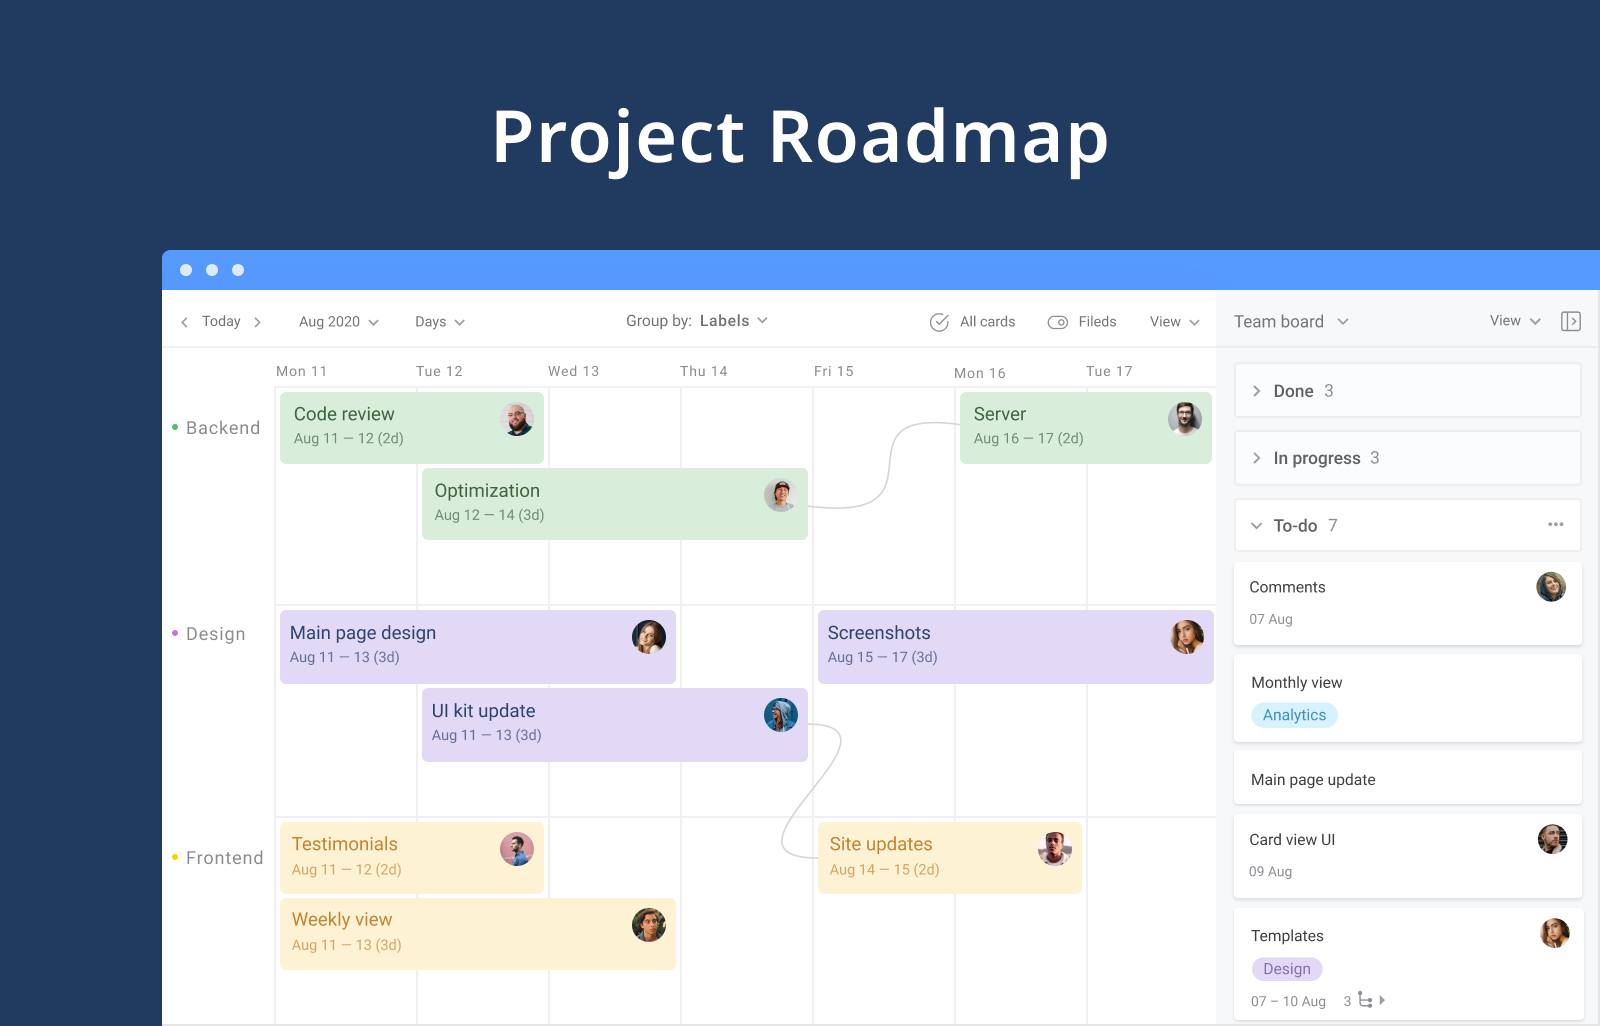
\includegraphics[width=0.8\linewidth]{images/trello_time_plan.png}
\caption{Project time plan}
\label{fig:timeplan}
\end{figure}
\newpage

\printbibliography
\end{document}
